\chapter{SUMMARY AND FUTURE WORK}
\label{chap:summary}
%
This dissertation presents a novel framework which enables remote workload
offloading to trusted remote computing resources through the
paradigm of extended hardware-layer heterogeneous computing environment.
%
Thus, the proposed framework broadens the range of heterogeneous
computing to remote resources in the network, where offloading services
are dynamically discovered. 
%
The proposed approach accomplishes this by extending the OpenCL framework to
support remote offloading using the TCP/IP networking stack and 
introducing the concept of Social Device Networks in which trusted
peers' computing resources are aggregated through virtual private
network for the purpose of resource discovery and configuration.
%
More specifically, the proposed framework is implemented as a wrapper
library around the OpenCL API with identical interfaces of the 
original library.
%
Furthermore, the wrapped library is integrated with a customized RPC-based
service to support remote offloading.
%
According to the decision from a runtime scheduler, each wrapped OpenCL API call
can invoke the corresponding original API in the local OpenCL library, or it
can be marshalled and sent to external resources for remote
execution.\\
%
Additionally, the proposed approach supports accessing remote resources beyond
the local private network, broadening the accessibility to trusted
remote resources across the Internet and the cloud.
%
This is accomplished by utilizing a social peer-to-peer virtual private
network, SocialVPN, and creating Social Device Network in which only
trusted social peers' computing resources are involved.
%
Also, the IP multicast-based resource discovery technique makes it possible
for mobile devices to dynamically discover remote resources during
runtime and to flexibly utilize computing capabilities of the remote resources.
%
With the proposed framework, therefore, a mobile device dynamically
discovers trusted remote resources in Social Device Network using the IP
multicast-based resource discovery mechanism, transparently offloads 
mobile workloads onto selected remote resources, and efficiently manages 
its energy consumption.\\   
%
For the second contribution of this dissertation, I analyzed the
behavior of the mobile offloading framework in terms of the offloading
performance and energy implication of the mobile device with respect to
workload and resource characteristics such as the size of data transfer,
workload complexity, network conditions or computing capabilities of
remote resources. 
%
In order to characterize mobile workloads, I utilized computation to
communication ratio calculated by local processing time divided by
time for data transfer.
%
Thus, in this dissertation, computation to communication ratio for each
workload is a comprehensive measurement which mirrors three parameters:
the volume of computations of workloads, the amount of data to be
transferred, and the network conditions.
%
I configured both local and wide area networks in which 
various computing capabilities are deployed to evaluate the impact of
resource characteristics into the offloading performance.
%
According to the analysis, the benefits and costs of remote
offloading depend on computation to communication ratio as well as
additional communications to setup extra arguments for workload
executions.
%
In fact, as computation to communication ratio becomes higher, 
the performance improvement and the conservation of energy consumption 
also increase.
%
Interestingly, in cases of hidden Markov model and {\it N}-body
physics, we observed that additional communications between the client
and server are also important to analyze the behavior of remote offloading 
for mobile platforms.\\
%
Then, I proposed a machine learning-based runtime scheduler for
mobile offloading framework.
%
In order to examine the feasibility of applying machine learning
techniques to adaptive scheduling problems for mobile offloading
framework, I evaluated well-known machine learning algorithms 
using Weka, a Java-based open source package.
%
To this end, I used computation to communication ratio, which represents
the local processing time for the workload and the amount of data transfer,
and network bandwidth, as attributes of the machine learning
technique.
%
After investigating the scheduling accuracy of several machine learning
algorithms, I chose a few machine learning algorithms which
have relatively high scheduling accuracy to implement offline
offloading schedulers.
%
In the evaluation, I showed that even though Instance-Based Learning 
offloading scheduler is fairly simple and has low overhead in terms of
algorithm complexity, it provides performance advantages over
non-adaptive scheduling policy as well as other machine learning-based
schedulers such as RandomTree or Rule-Based Learning.
%
In fact, the scheduler based on Instance-Based Learning
performed 7\% better than RandomTree and 3\% better than Rule-Based
Learning.\\
%
Next, I proposed a novel framework for an adaptive runtime scheduler for
mobile offloading by employing online machine learning techniques.
%
Particularly, this framework provides an online training mechanism for
the machine learning-based runtime scheduler such that it supports a
policy that dynamically adapts scheduling decisions at runtime based
upon the observation of previous offloading decisions and their
correctness.
%
Therefore, the proposed scheduling framework does not have to rely on any
predefined static scheduling policies or application-dependent
parameters.
%
To demonstrate its practical applicability, I integrated the proposed
framework with an existing Java-based, offloading-capable code
refactoring framework, DPartner.
%
The evaluation presents that the proposed work shows 10.9$\sim$40.5\%
higher scheduling accuracy than two static scheduling policies:
threshold-based and linear equation-based scheduling cases, according to
the computational complexity of applications and computing capability of
remote resources.\\
%
Lastly, I described a possible collaboration of mobile offloading
framework with the network proximity-aware clustering system by
introducing SOLARE, a peer-to-peer, utility functions based
self-organizing network latency-aware clustering system.
%
Since the main goal of SOLARE is to organize a proximity-aware
clustering topology, I believe that it is possible to provide mobile
offloading framework with more resilient resource discovery service by
supplying a list of remote resource which have similar network
performance.\\
%

%Furthermore, by taking the complexity and scheduling performance into
%account, I selected Instance-Based Learning algorithm for an online
%scheduler for mobile offloading framework.
%
%Using Instance-Based Learning online scheduler, I demonstrated
%the potential benefits and the ability of the online offloading
%scheduler to adapt to dynamic network conditions.\\
%
%Since the resource discovery of the proposed remote offloading framework
%is carried out on top of Social Device Network, the discovery scope
%can be limited within the user-defined virtual private network, and the
%remote resources, which are discovered through the resource discovery
%mechanism, enforce security and privacy in communication.
%
%Nevertheless, the resource selection among the discovered resources
%plays a critical role in quality of service for the application layer
%and user's mobility.
%
%In the current implementation, however, the process to select a
%remote resource is overly simple by employing only network latency as a
%main criterion for selecting the best remote resource.
%
%For future work, the current resource discovery technique will be 
%further extended into the consideration of keeping track of a more
%complex set of conditions of multiple remote computing resources such as
%network latency, bandwidth, and computing capabilities of remote
%resources, and the provision of the most appropriate resource in
%accordance with network conditions and mobile application requirements.
%
%Also, the machine learning-based runtime scheduler will be modularized
%so that it provides well-defined APIs, and the proposed runtime scheduler
%can be plugged and played for various types of adaptive scheduling
%problems.
%
%As part of the modularization of the machine learning-based runtime
%scheduler, I am currently working on the online scheduler for Java-based
%on-demand code offloading system.
%
%\section{On-Demand Resource Discovery and Selection}
%\label{summary:selection}
%
%\begin{figure}
%\centering
%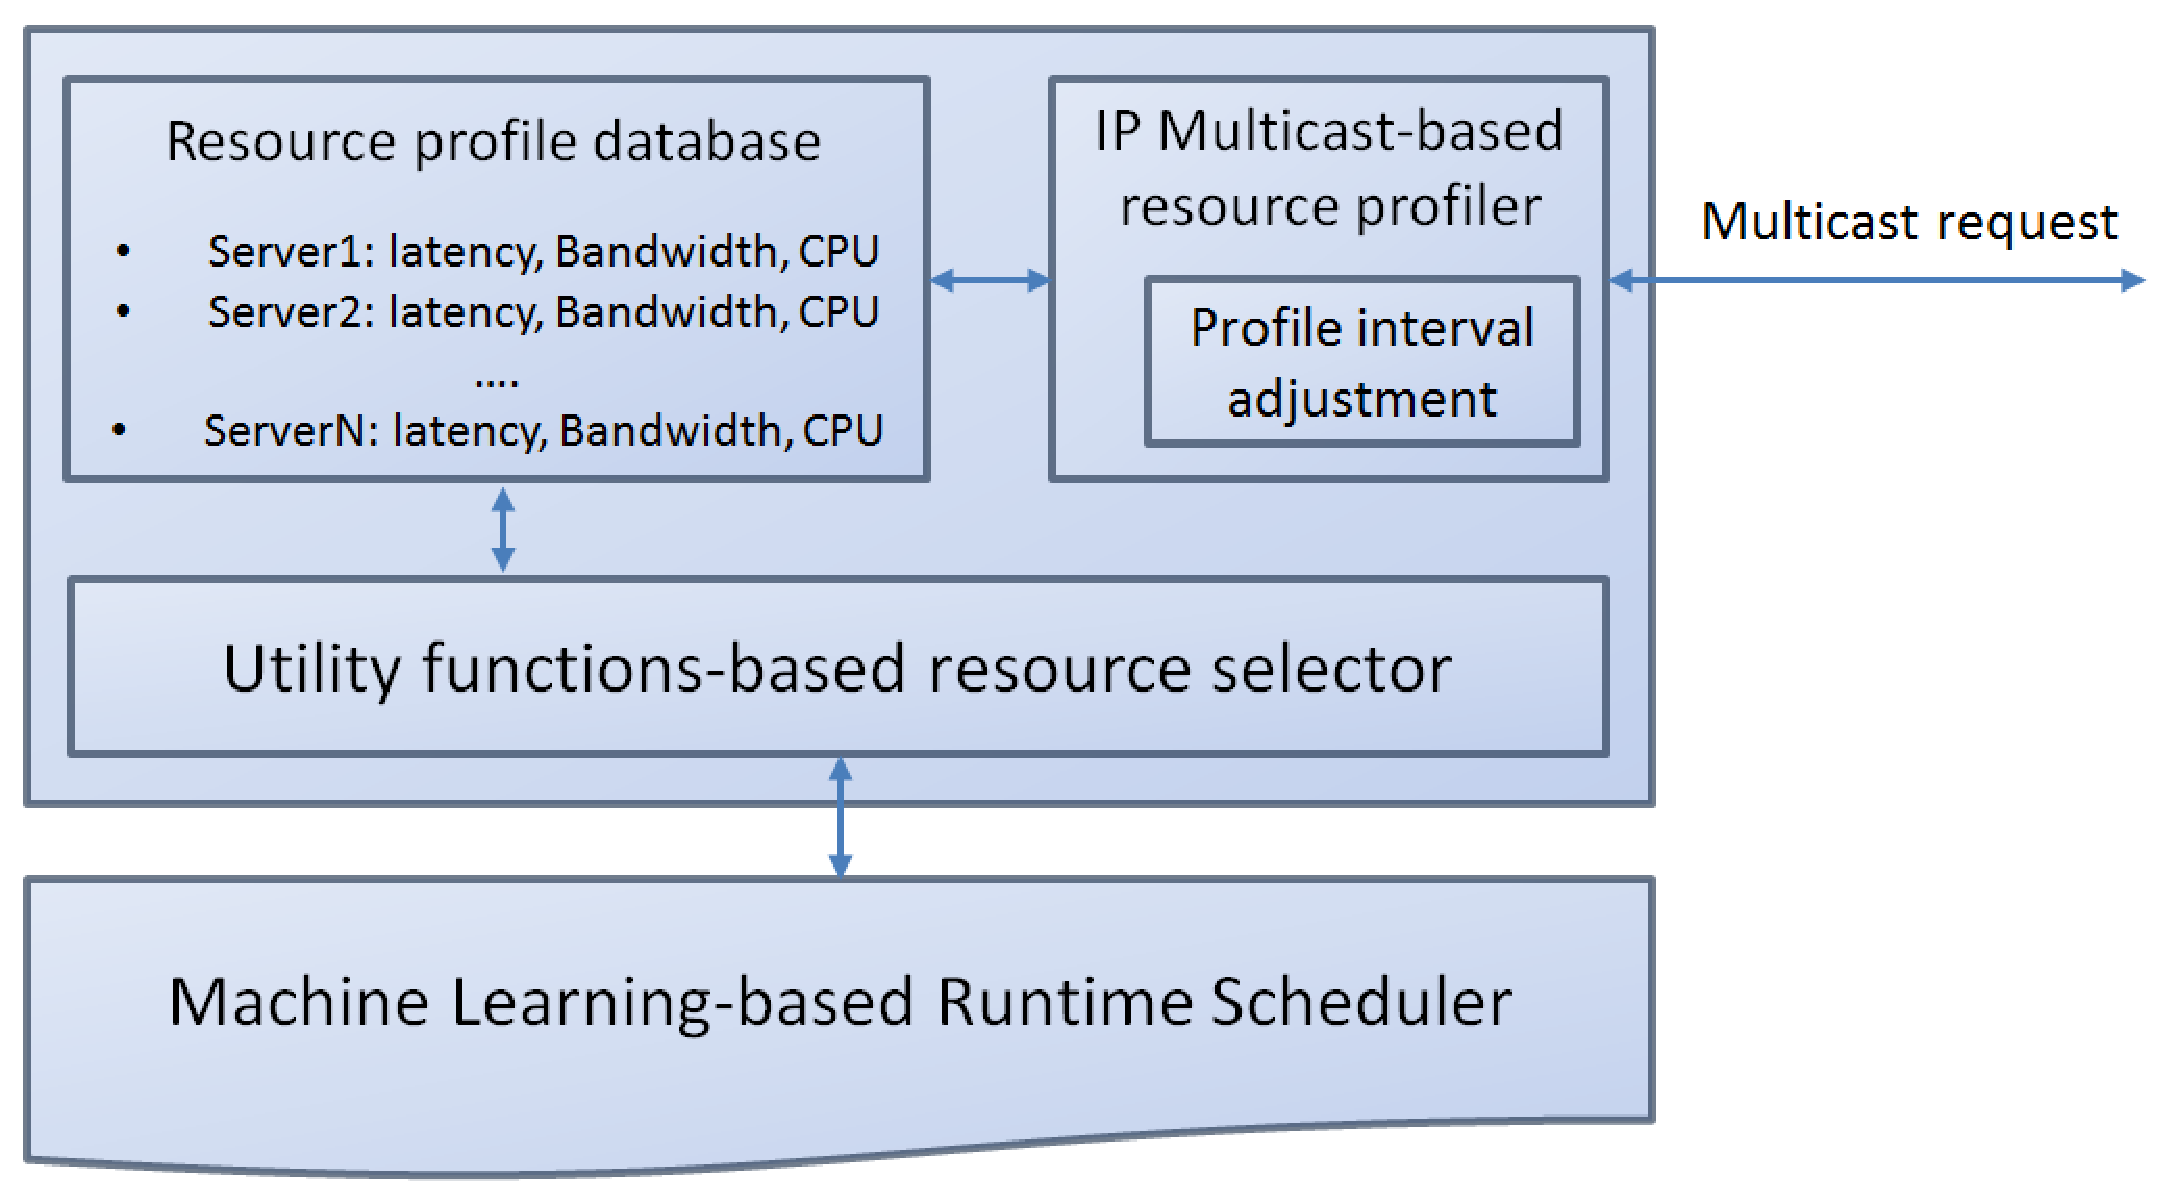
\epsfig{file=figs/ondemand.eps, width=4.0in}
%\caption{Structure of on-demand resource discovery and selection
%mechanism}
%\label{fig:ondemand}
%\end{figure}
%
Service discovery protocols make developers free from taking care of all
possible interactions and states between devices at design time by
including a layer of indirection to remote offloading
framework~\cite{feng}.
%
However, it is still challenging to define a discovery scope when the
offloading framework is deployed in wide area environments rather than
in local area environments such as enterprise networks protected by
firewalls and managed by system administrators.\\
%
The IP multicast-based resource discovery over Social Device
Network, which is accomplished through a peer-to-peer virtual private network,
SocialVPN, can limit the discovery scope within the user-defined virtual
private network, thus, the discovered remote resources enforce security
and privacy in communication.
%
Nevertheless, it is crucial that a proper policy for the resource
selection needs to provide the most appropriate resource among the discovered
remote resources in accordance with network conditions and application
characteristics to offer quality of service for the application layer
and the elasticity for the user's mobility. 
%
The default behavior of the current implementation of the resource 
discovery mechanism is to profile available remote resources and 
provide the one with the lowest network latency only when a workload 
is needed to be offloaded.
%
As a result, the process to select a remote resource is overly simple by
employing only network latency as a main criterion for selecting the
best resource, and it is difficult to capture the sophisticated set of
information for remote resources.
%
Furthermore, in the mobile computing environment, as the physical
location of mobile hosts can be changed from time to time and
network access points might be changed as well, it is essential to take the
mobility into account and it is required to have more fine-grained
resource profiling and selection mechanism.\\
%
\begin{figure}
\centering
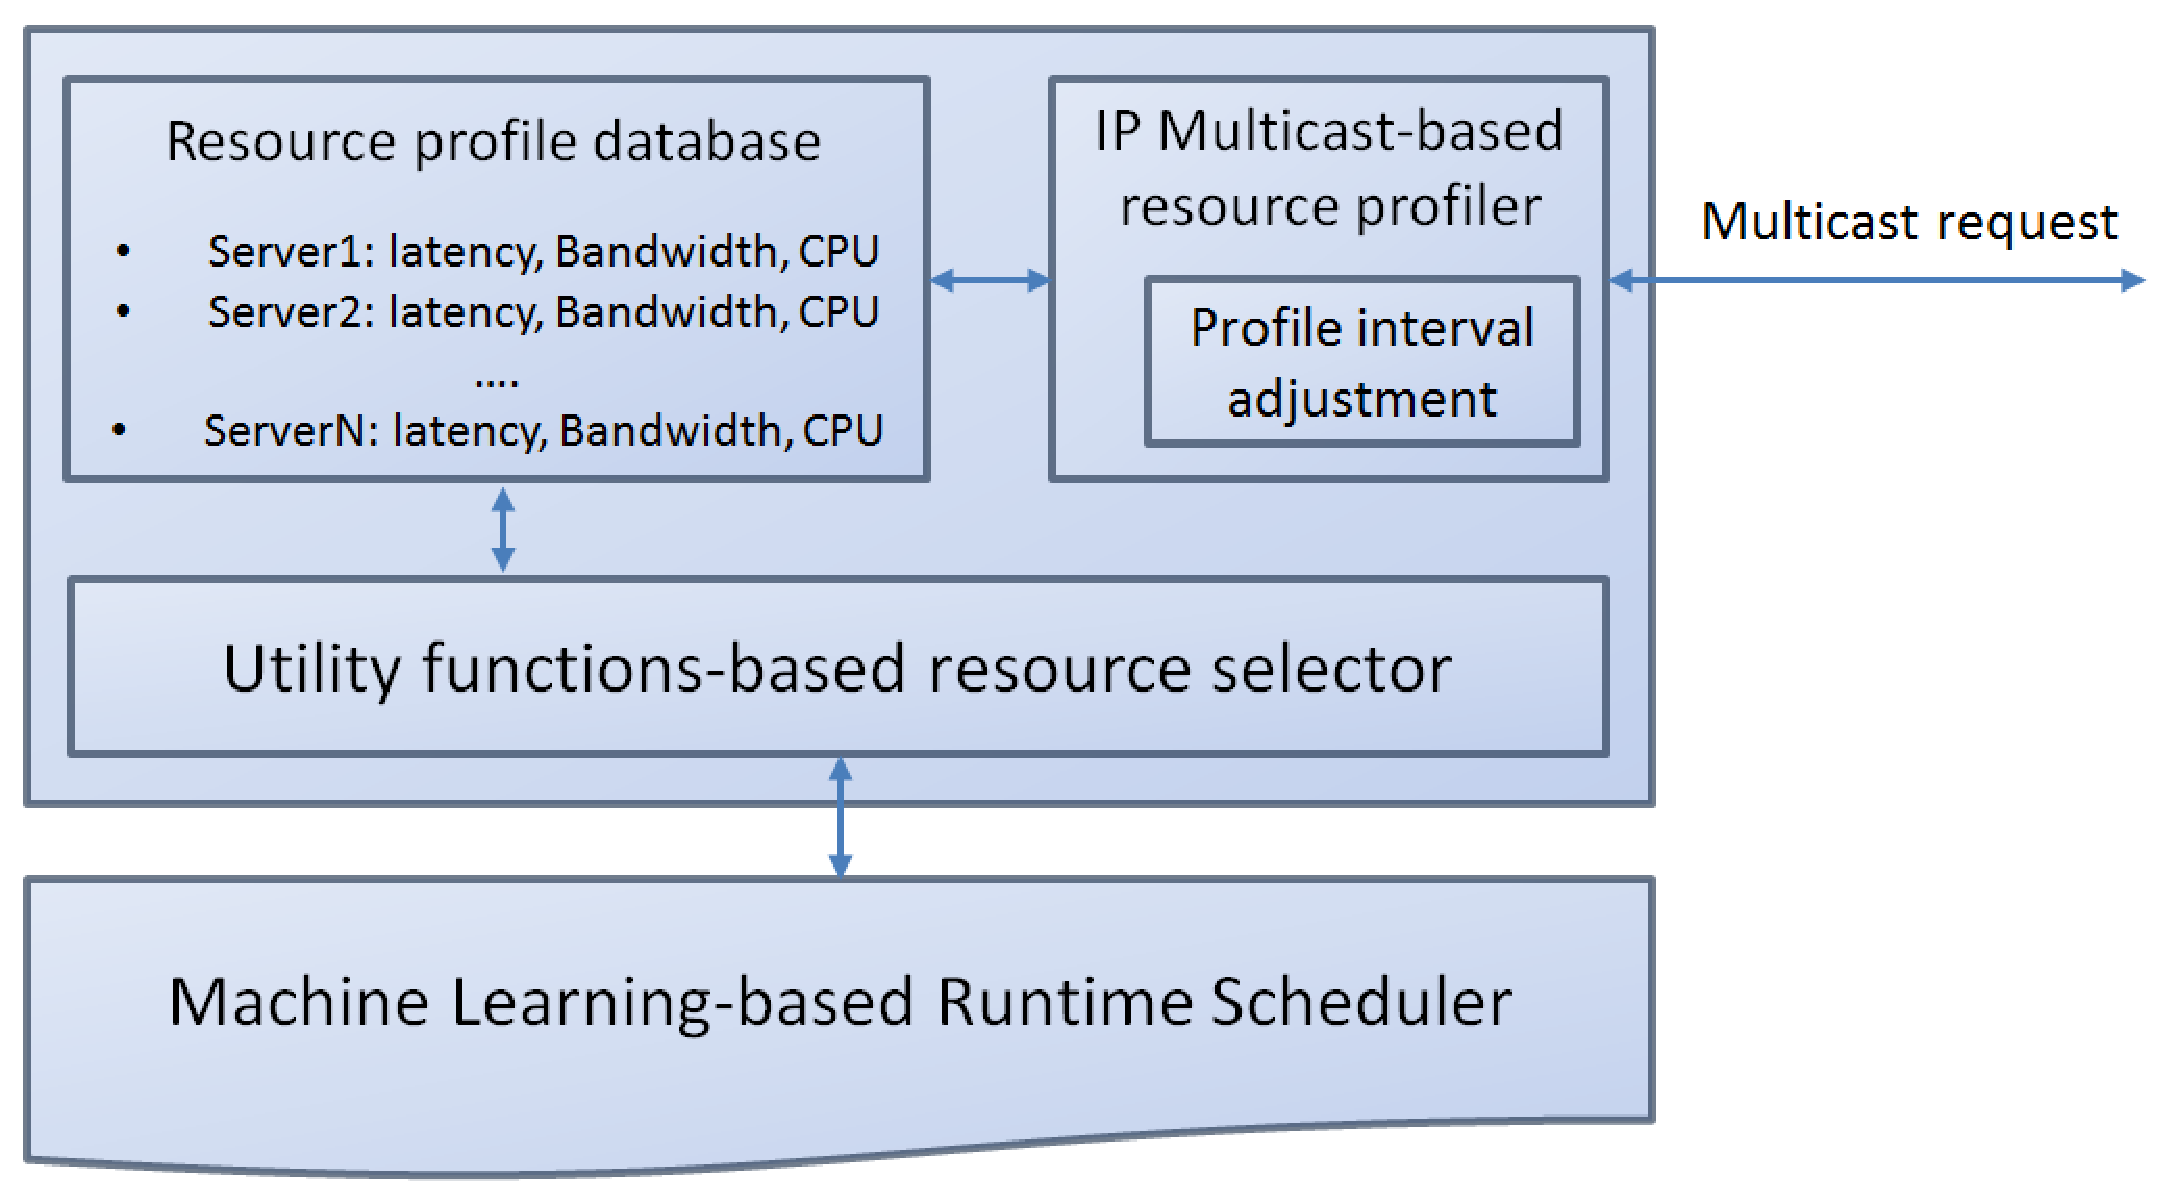
\epsfig{file=figs/ondemand.eps, width=4.0in}
\caption{Structure of on-demand resource discovery and selection
mechanism}
\label{fig:ondemand}
\end{figure}
%
As a next goal of the future work, I plan on extending the current resource 
discovery technique into a more fine-grained resource discovery technique in 
which a more complex set of conditions will be periodically monitored and the
most appropriate remote resource will be selected in accordance with
application characteristics and requirements.
%
To this end, I propose a fine-grained on-demand resource discovery and
selection approach that can automatically make the resource selection which would
yield the best performance without any user interventions.
%
Even though there exist many ways to achieve the automatic
resource selection, a utility functions-based approach can be used due to
its expressiveness of preference and ability of self-optimization.
%
Utility functions provide a natural and advantageous framework for
achieving self-optimization in autonomic computing by representing user
or application preference~\cite{utility}.
%
For that reason, utility functions have been applied to autonomic systems,
particularly, to the resource allocation in high performance computing
environments~\cite{william, david, terence, paul}.
%
Thus, by implementing utility functions-based on-demand resource
selection with various features such as latency, bandwidth, or computing
capabilities of remote resources, and by setting different weight values
of each feature for utility functions in accordance with application
characteristics and requirements, it is expected that the proposed
resource discovery technique provides a more flexible capability of
selecting the appropriate resource according to application expectations
and preference priority.\\
%
Figure~\ref{fig:ondemand} shows the structure of the proposed on-demand 
resource discovery and selection mechanism. 
%
The IP multicast-based resource discovery profiles remote
resources involved in a social device network by periodically sending
multicast request packets with a certain interval.
%
It is worth noting that the interval for request packets is adaptively
changed according to network conditions.
%
If network conditions such as latency or bandwidth have high variance,
the request rate increases so that the information for remote resources 
can be updated sufficiently often.
%
%the request rate increases so that the resource profile database keeps
%the information for remote resources up to date.
%
Otherwise, the resource discovery stays in a low request rate to save
energy consumption of a mobile client. 
%
Whenever the machine learning-based runtime scheduler requests a remote
resource, the utility functions based resource selector delivers the
remote resource which has the highest utility value to the runtime
scheduler along with its information such as network performance or
computing capabilities.\\
%
\begin{figure}
\centering
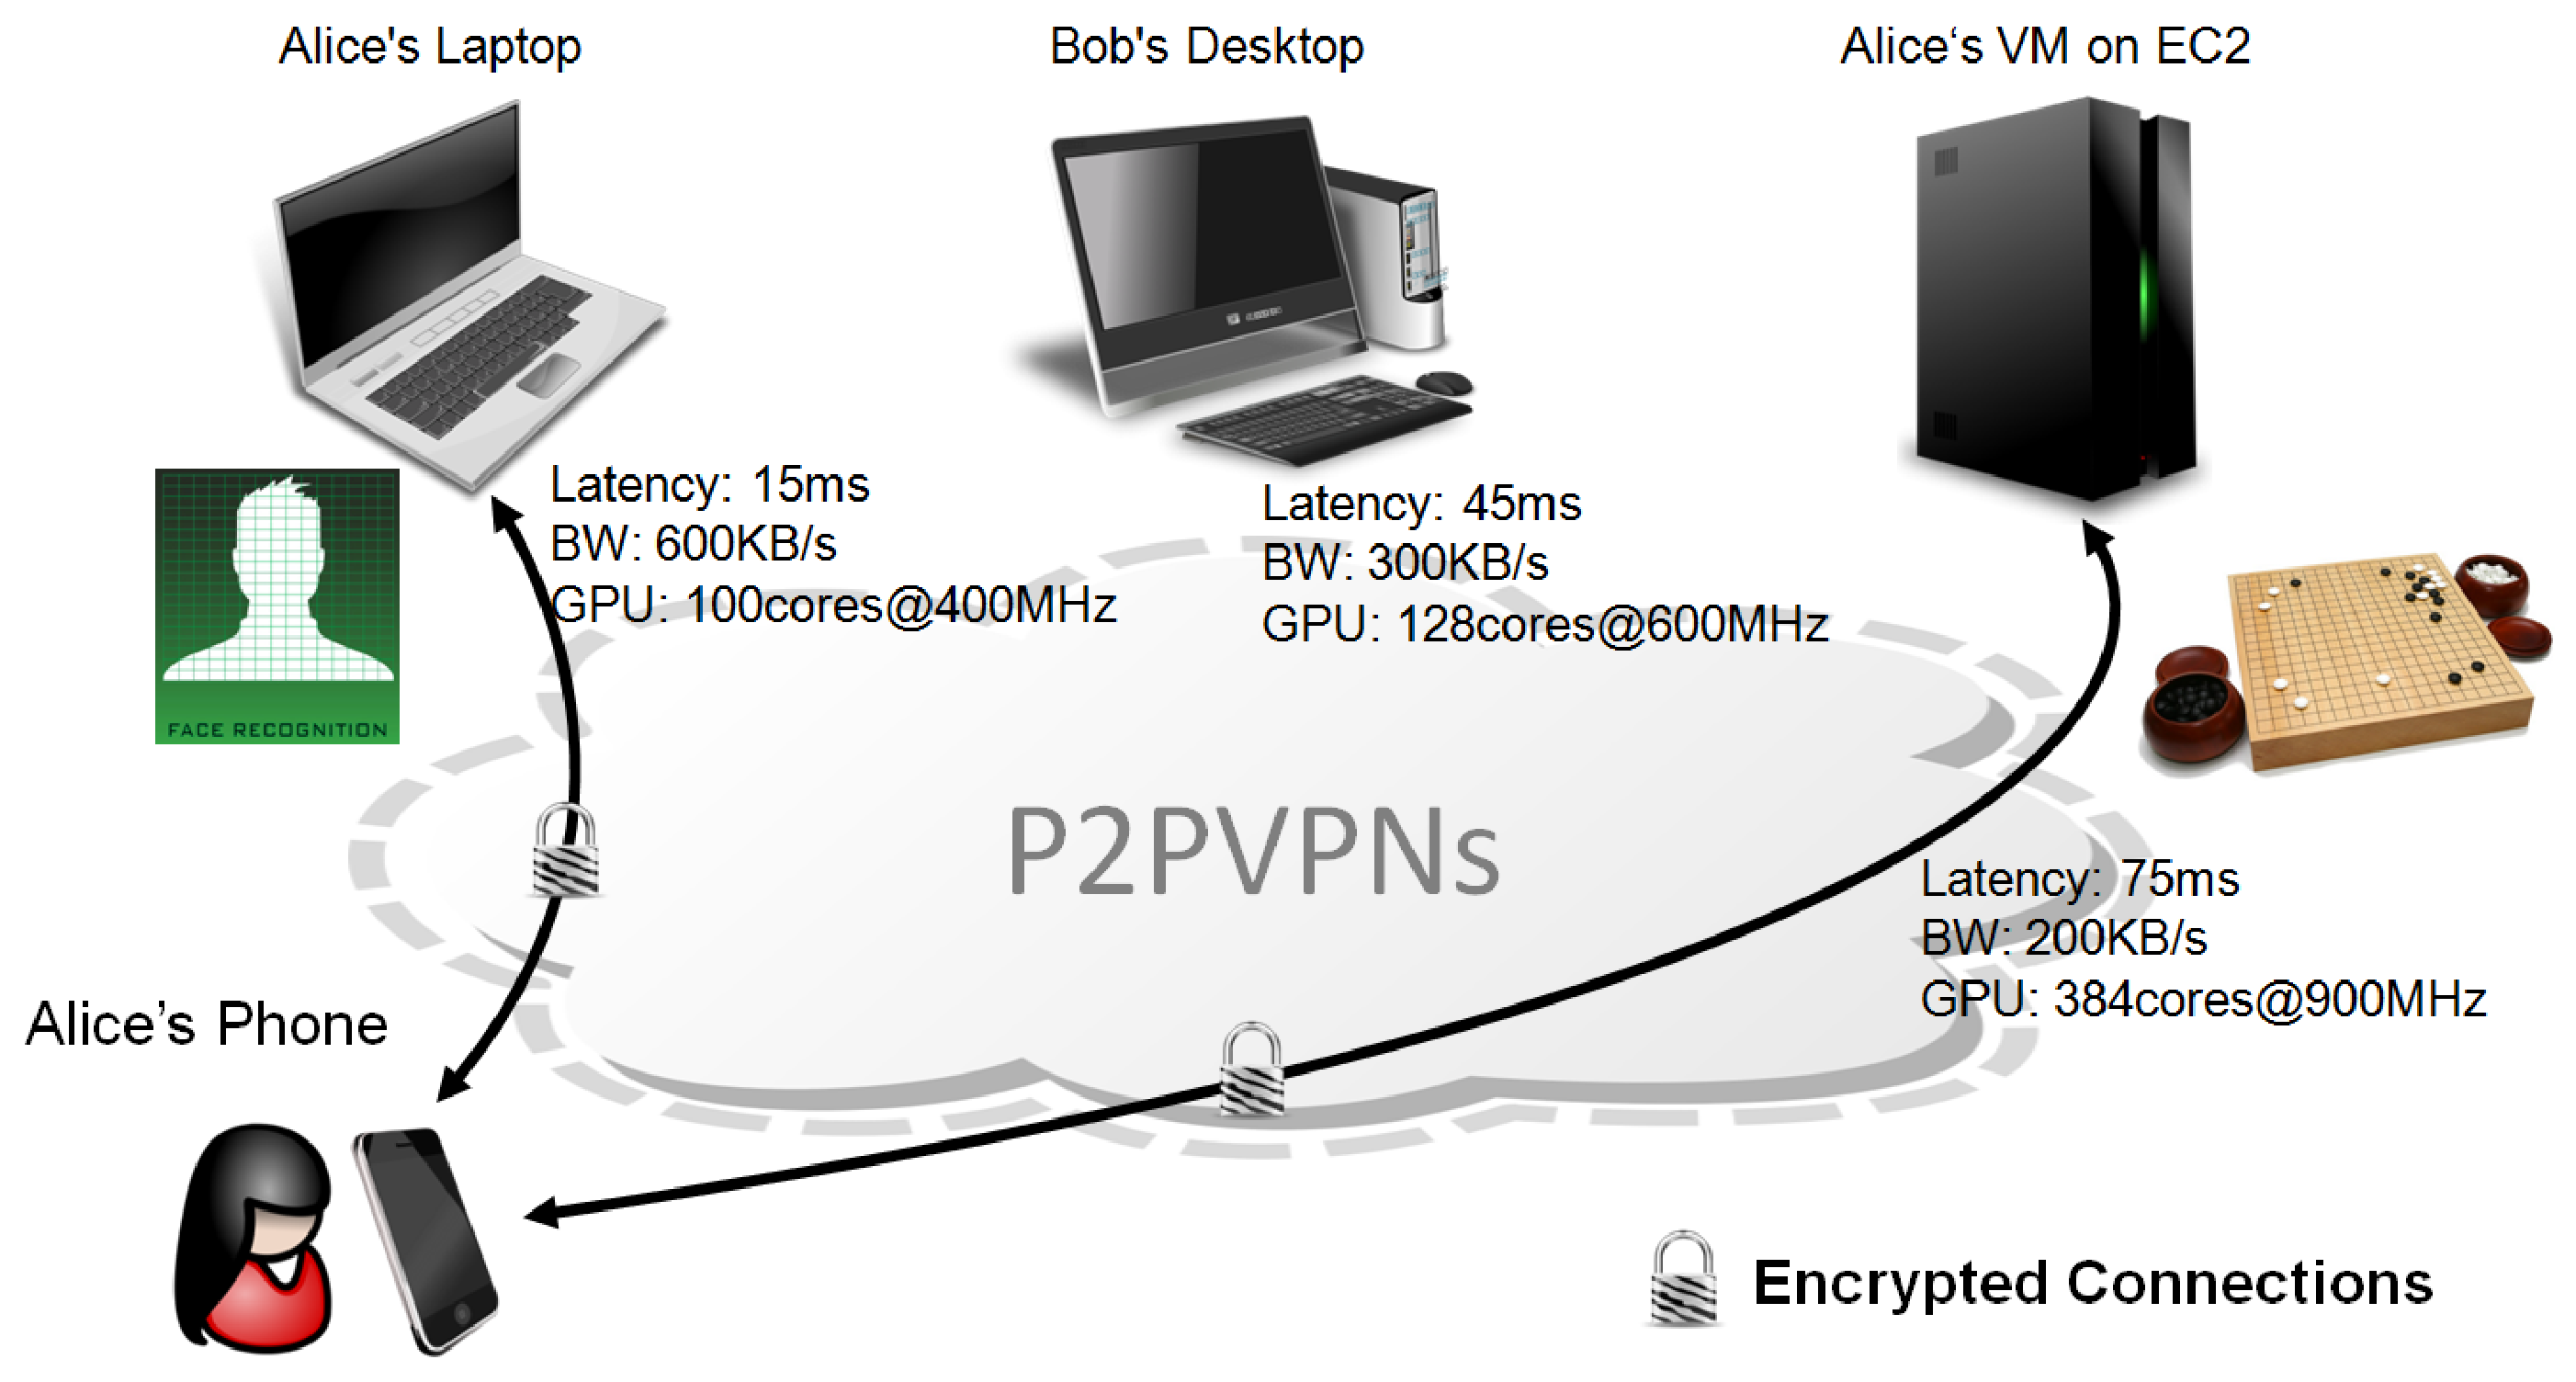
\epsfig{file=figs/futurework.eps, width=5.5in}
\caption{On-demand resource discovery and selection}
\label{fig:futurework}
\end{figure}
%
Figure~\ref{fig:futurework} illustrates a typical use case scenario of
the utility functions-based on-demand resource discovery and selection
technique.
%
First, Alice considers two different types of mobile applications, first
application recognizes the face of human being from a video clip and
second application is a Go game in which the mobile user plays
the game with virtual competitor.
%
For first application, it is required that large amounts of data should
be transferred from the mobile device to the remote resource as the
application processes through a series of images.
%
Therefore, it might be most important that network bandwidth between the
mobile device and the remote resource should be high enough to support
the seamless service of the face recognition.
%
As a result, the on-demand resource selection mechanism will select
Alice's laptop as a target resource which has the highest bandwidth
among three remote resources.
%
For the Go game, on the other hand, the mobile device transfers only
several hundreds of bytes of data which present current positions of
stones and the remote resource calculates the optimal next stone
position with certain complex algorithms such as Monte Carlo or pattern
matching.
%
Consequently, the resource selection mechanism selects the most powerful
computing resource, Alice's VM on EC2, even though it has the worst
network performance.\\
%
The proposed on-demand resource selection based on utility functions
will be evaluated through real deployment into various network
configurations which have different network performance in terms of
latency and bandwidth.
%
Furthermore, in order to examine the ability of on-demand resource
selection, I will utilize different types of mobile applications which
have different characteristics and requirements such as image
processing, character recognition, and gaming systems.
%

%\section{Performance Characterization of ML-based Runtime Schedulers}
%\label{summary:scheduler}
%
%\begin{figure}
%\centering
%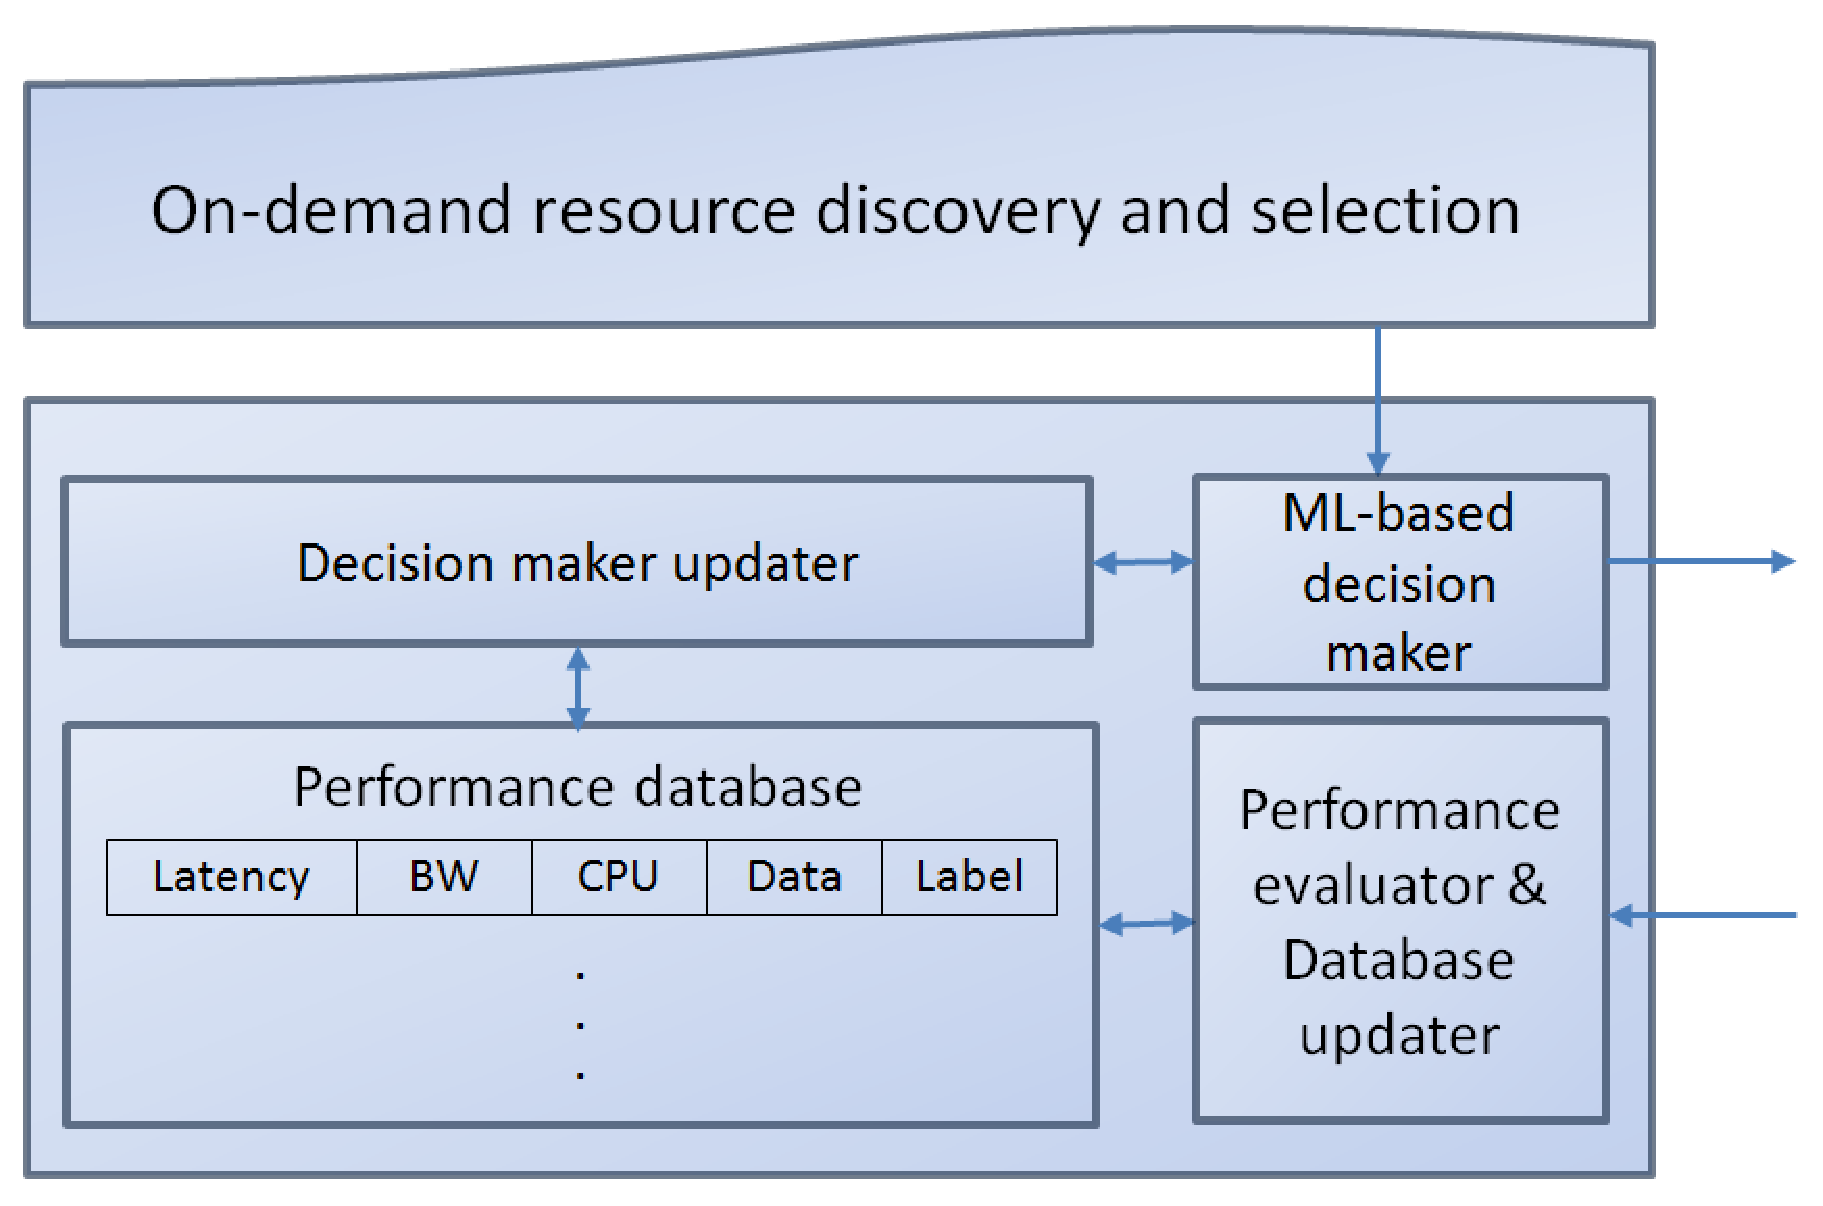
\epsfig{file=figs/mlscheduler.eps, width=4.0in}
%\caption{Modularization of the machine learning-based runtime scheduler}
%\label{fig:mlscheduler}
%\end{figure}
%
%In the evaluation of the machine learning-based runtime scheduler, it
%has been shown that several machine learning algorithms such as
%Instance-Based Learning or RandomTree have potential benefits and the
%ability of the on/offline offloading scheduler to adapt into dynamic
%network conditions and application requirements.
%
%However, the current prototype of the machine learning-based runtime
%scheduler has been implemented upon the OpenCL-based remote offloading
%framework and it uses the OpenCL-dependent parameter, the number of the
%invocations for argument setup API (i.e. clSetkernelArgs({\it
%n$_{argset}$})), as an
%attribute of machine learning algorithms.
%
%Therefore, it is impractical to apply the proposed machine
%learning-based runtime scheduler into different types of remote
%offloading systems which have a different set of features to represent
%the scheduling problem.
%
%For a next goal for the machine learning-based runtime scheduler, I will
%generalize and modularize the components of the machine learning-based
%runtime scheduler which is shown in Figure~\ref{fig:scheduler} and
%provide the well-defined APIs so that various offloading frameworks can
%easily take the advantages of the machine learning-based runtime
%scheduler.
%
%For example, API, {\it getAttributes()} gives developers the
%functionality which takes the profiled information for network
%conditions and application characteristics as input parameters and
%generates a set of attributes used by the machine learning-based
%classifier to make the final decision to offloading or local execution.
%
%Also, it is possible to implement several types of ML-based classifiers
%with different machine learning algorithms so that the developer can
%build the attribute-dependent runtime scheduler.
%
%Figure~\ref{fig:mlscheduler} details the modularization of the machine
%learning-based runtime scheduler.
%
%First, the machine learning-based decision maker takes the information
%of the selected resource and makes a decision the workload is offloaded
%or executed in local.
%
%Next, the offloading performance will be evaluated by the performance
%evaluator and the database updater will update the performance database.
%
%Based on the updated database, the decision maker updater will update
%the machine learning-based decision maker.\\
%
%One of the contributions of the modularization of the machine
%learning-based runtime scheduler is to characterize the performance,
%benefits and overhead of different types of machine learning algorithms
%in mobile offloading online scheduler scenario.
%
%As presented in section~\ref{chap:scheduler}, while the machine
%learning techniques show the feasibility of applying to the runtime
%scheduler for mobile offloading framework, different types of 
%machine learning algorithms vary considerably in the performance 
%and costs for the runtime offloading scheduler.
%
%It is effective to identify the performance, benefits and costs of
%different types of machine learning algorithms in online scheduler
%scenario.
%
%To my best knowledge, it is first to consider the characterization of
%machine learning algorithms for the runtime mobile offloading
%scheduler.\\
%
%As part of the modularization of the machine learning-based runtime
%scheduler, I am currently working for transplanting the modules of the
%machine learning-based runtime scheduler into on-demand Android Java
%code offloading framework~\cite{dpartner}.
%
%In the current implementation for on-demand Android Java code offloading
%framework, the task to scheduler code offloading is completely dependent
%on a mobile user's control.
%
%In fact, the on-demand Java code offloading system depends on the 
%web-based user interface called RuntimeManager in which a mobile user
%schedules each offloadable class by dragging and dropping the badges 
%representing offloadable classes into local and remote area in 
%RuntimeManager.
%
%As a result, this scheduling policy of the Java on-demand offloading
%system does not consider network conditions and application requirements
%at all and the mobile user can make wrong scheduling which might cause
%poor application performance and unnecessary energy consumption.\\
%
%By placing the module of the machine learning-based runtime scheduler
%and implementing the online scheduler based on machine learning
%techniques into the client side of Android Java code offloading
%framework, it will dynamically profile network conditions and
%application requirements, and user-transparently decide offloading or
%local execution in accordance with the previous offloading performance.
%
